
\section{Simplified geometry experiments with PISM}\label{sec:simp}

\subsubsection*{Historical note}  There have been three stages of ice sheet model intercomparisons based on simplified geometry experiments since the early 1990s \cite{BuelerSpray}.\index{EISMINT!defined}

EISMINT I \cite[ European Ice Sheet Modeling INiTiative]{EISMINT96}\footnote{See \url{http://homepages.vub.ac.be/\%7Ephuybrec/eismint.html}.} was the first of these and involved only the isothermal shallow ice approximation (SIA).  Both fixed margin and moving margin experiments were performed in EISMINT I, and various conclusions were drawn about the several numerical schemes used in the intercomparison.  EISMINT I is superceded, however, by verification using the full variety of known exact solutions to the isothermal SIA \cite{BLKCB}.  The ``rediscovery'', since EISMINT I, of the Halfar similarity solution with zero accumulation \cite{Halfar83}, and verification runs using that solution, already suffices to measure the isothermal SIA performance of PISM more precisely than would be allowed by comparison to EISMINT I results.

EISMINT II \cite{EISMINT00} pointed out interesting and surprising properties of the thermocoupled SIA.  References \cite{BBL,Hindmarsh04,Hindmarsh06,PayneBaldwin,SaitoEISMINT,BBssasliding} each interpret the EISMINT II experiments and/or describe attempts to add more complete physical models to ``fix'' the (perceived and real) shortfalls of ice sheet model behavior on EISMINT II experiments.  We believe that the discussion in \cite{PayneDongelmans,PayneBaldwin,BBL} adequately explains the ``spokes'' in EISMINT II experiment F as a genuine fluid instability, while Appendix B of \cite{BBssasliding} adequately cautions against the continuum model that generates the ``spokes'' in EISMINT II experiment H.   Thus we can move on from that era of controversy.  In any case, PISM has built-in support for all of the published and unpublished EISMINT II experiments; these are described in the next subsection.

The ISMIP (Ice Sheet Model Intercomparison Project)\footnote{See \url{http://homepages.vub.ac.be/\%7Ephuybrec/ismip.html}.}\index{ISMIP!defined} round of intercomparisons is still ongoing at this time (2009).  There are two components of ISMIP substantially completed, namely HOM = Higher Order Models \cite{ISMIPHOM,HOMelmer} and HEINO = Heinrich Event INtercOmparison \cite{GreveTakahamaCalov,Calovetal2009HEINOfinal}.  Of these, PISM participated in HEINO, but this ability is unmaintained.   We believe\index{ISMIP!interpretation of HEINO results} the continuum problem described by HEINO, also used in EISMINT II experiment H (above), is not easily approximate-able because of a required discontinuous jump in the basal velocity field.  The continuum problem predicts infinite vertical velocity because of this jump \cite[Appendix B]{BBssasliding}.  Details of the numerical schemes and their results are irrelevant if the continuum model makes such a prediction.

PISM offers the physical continuum model described in \cite{BBssasliding}, an SIA/SSA hybrid, as an alternative to the continuum model used in ISMIP-HEINO and EISMINT II experiment H.  Indeed the SIA/SSA hybrid is offered as a unified shallow model for real ice sheets (section \ref{sec:dynamics}).

There is no current plan to support ISMIP-HOM, but comparison of shallow PISM results to exact Stokes solutions is a goal for PISM evaluation.

A third ISMIP part is the Marine Ice Sheet Model Intercomparison Project (MISMIP)\index{ISMIP!MISMIP}.  It is minimally supported in PISM, as described in subsection \ref{subsect:MISMIP} below.


\subsection{EISMINT II}\label{subsect:EISMINTII}
\optsection{EISMINT II}

There are seven experiments described in the published EISMINT II writeup \cite{EISMINT00}.\index{EISMINT}  They are named A, B, C, D, F, G, and H.  They have these common features:\begin{itemize}
\item runs are for 200,000 years, with no prescribed time step;
\item a $61\times 61$ horizontal grid on a square domain ($1500$ km side length) is prescribed;
\item the surface inputs (temperature and mass balance) have angular symmetry around the center of the grid;
\item the bed is flat and does not move (no isostasy);
\item the temperature in the bedrock is not modeled;
\item only the cold (not polythermal) thermomechanically-coupled shallow ice approximation is used \cite{EISMINT00}; and
\item though basal melt rates may be computed diagnostically, they do not affect the evolution of the ice sheet.
\end{itemize}
The experiments differ from each other in their various combinations of surface temperature and mass balance parameterizations.  Experiments H and G involve basal sliding, under the physically-dubious SIA sliding rubric \cite[Appendix B]{BBssasliding}, while the others don't.  Four experiments start with zero ice (A,F,G,H), while the other experiments (B,C,D) start from the final state of experiment A.

In addition to the seven experiments published in \cite{EISMINT00}, there were an additional five experiments described in the EISMINT II intercomparison description 
\cite{EISIIdescribe}, labeled E, I, J, K, and L.\index{EISMINT!unpublished additional EISMINT II experiments}  These experiments share most features listed above, but with the following differences.  Experiment E is the same as experiment A except that the peak of the accumulation, and also the low point of the surface temperature, are shifted by 100 km in both $x$ and $y$ directions; also experiment E starts with the final state of experiment A.  Experiments I and J are similar to experiment A but with non-flat ``trough'' bed topography.  Experiments K and L are similar to experiment C but with non-flat ``mound'' bed topography.

See table \ref{tab:eisII} for how to run all EISMINT II experiments in PISM.  Note that the vertical grid is not specified in EISMINT II, and it seems that good simulation of the thermomechanically-coupled conditions near the base of the ice requires relatively-fine resolution there.  (It is difficult to be quantitative because of a lack of theory.)  We suggest using the default unequally-spaced grid with 61 levels, which gives a grid spacing of 21 m in the ice layer closest to the bed.\footnote{An equally-spaced grid is an option in PISM, and in this case we suggest using 201 vertical levels to give 25 m spacing.}

These SIA-only simulations parallelize particularly well.  Very roughly, for the standard $61\times 61$ horizontal grid, wall-clock-time speedups will occur up to about 30 processors, and finer grids will benefit from even more processors, of course.

Table \ref{tab:eisII} shows how all EISMINT II experiments are done in PISM.  Experiments below the horizontal line in Table \ref{tab:eisII} are only documented in \cite{EISIIdescribe}.

\begin{table}[ht]
\centering
\small
\begin{tabular}{@{}llll}\toprule
\textbf{Command: ``\texttt{pisms }'' $+$} & \textbf{Relation to experiment A} \\
\midrule
\texttt{-eisII A -Mx 61 -My 61 -Mz 61 -y 200000 -o eisIIA.nc} & \\
\texttt{-eisII B -i eisIIA.nc -y 2e5 -o eisIIB.nc} & warmer \\
\texttt{-eisII C -i eisIIA.nc -y 2e5 -o eisIIC.nc} & less snow (lower accumulation)\\
\texttt{-eisII D -i eisIIA.nc -y 2e5 -o eisIID.nc} & smaller area of accumulation \\
\texttt{-eisII F -Mx 61 -My 61 -Mz 61 -y 2e5 -o eisIIF.nc} & colder; famous spokes \cite{BBL} \\
\texttt{-eisII G -Mx 61 -My 61 -Mz 201 -y 2e5 -o eisIIG.nc} & sliding (regardless of temperature) \\
\texttt{-eisII H -Mx 61 -My 61 -Mz 201 -y 2e5 -o eisIIH.nc} & melt-temperature activated sliding \\ \midrule
\texttt{-eisII E -i eisIIA.nc -y 2e5 -o eisIIE.nc} & shifted climate maps \\
\texttt{-eisII I -Mx 61 -My 61 -Mz 201 -y 2e5 -o eisIII.nc} & trough topography \\
\texttt{-eisII J -i eisIII.nc -y 2e5 -o eisIIJ.nc} & trough topography and less snow \\
\texttt{-eisII K -Mx 61 -My 61 -Mz 201 -y 2e5 -o eisIIK.nc} & mound topography \\
\texttt{-eisII L -i eisIIK.nc -y 2e5 -o eisIIL.nc} & mound topography and less snow \\
\bottomrule
\normalsize
\end{tabular}
\label{tab:eisII}
\caption{Running the EISMINT II experiments in PISM.\index{PISM!running the EISMINT II experiments in}  Use \texttt{-skip -skip_max 5}, on the $61\times 61$ default grid, for significant speedup.}
\end{table}

The EISMINT II experiments can be run with various modifications of the default settings.  Of course the grid can be refined.  For instance, a twice as fine grid in the horizontal is ``\texttt{-Mx 121 -My 121}''.  Table \ref{tab:eisIIoptions} lists some optional settings which are particular to the EISMINT II experiments.

\begin{table}[ht]
\centering
\small
\begin{tabular}{@{}lp{0.35\linewidth}lp{0.35\linewidth}}\toprule
\textbf{Option} & \textbf{Default values [expers]} & \textbf{Units} & \textbf{Meaning} \\\midrule
\intextoption{eisII} & A & &  Choose single character name of EISMINT II \cite{EISMINT00} simplified geometry experiment.  Allowed values are A, B, C, D, E, F, G, H. \\
\intextoption{Mmax} & 0.5 [ABDEFGHIK], 0.25 [CJL] & m$/$a & max value of accumulation rate \\
\intextoption{Rel} & 450 [ABEFGHIK], 425 [CDJL] & km & radial distance to equilibrium line \\
\intextoption{Sb} & $10^{-2}$ [\emph{all}] & (m/a)/km & radial gradient of accumulation rate \\
\intextoption{ST} & $1.67 \times 10^{-2}$ [\emph{all}] & K/km & radial gradient of surface temperature\\
\intextoption{Tmin} & 238.15 [ACDEGHIJKL], & K & max of surface temperature \\
 & 243.15[B], 223.15[F] & & \\
\intextoption{bmr_in_cont} & & & Include the basal melt rate in the mass continuity computation (override default for EISMINT II)\\
\bottomrule\normalsize
\end{tabular}
\label{tab:eisIIoptions}
\caption{Changing the default settings for EISMINT II}
\end{table}

In PISM the height of the computational box, the quantity set by \texttt{-Lz}, is set at the beginning of the run.  It is chosen for the EISMINT II experiments according to the observed maximum values occuring in standard runs.  If the ice thickens beyond the chosen level for the top of the computational box then additional layers are automatically added to the computational grid.  In fact, if the ice grows above the height of the computational box then a message appears, \texttt{PISM WARNING: max ice thickness ... is greater than the height of the computational box ...}, and then at least two additional levels are added to the vertical grid.  This is to some degree an emergency mechanism, however, because it can run away to use up all memory in extreme cases.  If the height of the computational box grows so large that the grid has more than twice the original number of vertical levels then PISM produces a \texttt{PISM ERROR} error message and stops.   Therefore it is possible that the number of vertical levels at the end of the run exceeds the initial \texttt{-Mz} value.  Setting EISMINT II options \texttt{-Mmax} or \texttt{-Sb} to produce higher accumulation rates than the default values (see table \ref{tab:eisIIoptions}) may cause the ice sheet to thicken above the standard thickness and therefore trigger this automatic extension mechanism.  Similarly, colder ice caused by nonstandard \texttt{-Tmin} or \texttt{-ST} values can produce unusually thick ice.  The user may always choose to use a larger, more conservative value for option \texttt{-Lz}, however.


\subsection{MISMIP}\label{subsect:MISMIP}
\optsection{MISMIP}

This intercomparison addresses grounding line dynamics by considering an idealized one-dimensional stream-shelf system.  The intercomparison process is described at the website

\centerline{\url{http://homepages.ulb.ac.be/~fpattyn/mismip/}}

\noindent Find a full text description there.  It is essential reading for understanding MISMIP results generally, and for appreciating many of the comments in this subsection.

PISM's version of MISMIP includes an attached ice shelf even though modeling the shelf is theoretically unnecessary in the MISMIP flow line case.  The analysis in \cite{SchoofMarine1} shows that the only effect of an ice shelf, in the flow line case, is to transfer the force imbalance at the calving front directly to the ice column at the grounding line.  But this analysis does not apply to ice shelves with two horizontal dimensions, of course.  Real ice shelves have ``buttressing'' and ``side drag'' and other forces not present in flow line circumstances \cite{Goldbergetal2009}.  See the Ross ice shelf example in section \ref{sec:ross}, for example.

We use the usual PISM ice shelf model, with two horizontal dimensions, to do MISMIP.  This intercomparison therefore looks at the grounding line dynamics results from the usual PISM code, though in a highly symmetric case without side drag.

Because PISM is a model with two horizontal dimensions, we must adapt it to do a flow line problem (see section \ref{sec:flowline-modeling}). The flow direction for MISMIP is arbitrarily taken to be ``$x$''.  We periodize the cross-flow direction ``$y$'', and use the minimum number of points in this direction which maintains function.  This number turns out to be ``\texttt{-My 3}''; fewer points than this in the cross-flow direction confuses the finite difference scheme.

PISM has two applicable ice dynamics models. Model 1 is a pure SSA model.  It is ``category 2'' in the MISMIP classification.  Model 2 combines SIA and SSA velocities as described in \cite{BBssasliding}, and is ``category 3'' because it resolves ``vertical'' shear (i.e.~using SIA flow).

There are many runs for a complete MISMIP intercomparison submission.  There are $62$ runs for each model and grid choice, and there are two models and three (suggested) grid choices, so a full suite is $6 \times 62 = 372$ runs.  The finest grid runs account for all the compute time, however.  ``Grid mode 2'' in the MISMIP description is 1500 grid spaces in the flow line direction\footnote{This translates into 3001 grid \emph{points} in PISM's doubled computational domain.}, a very fine grid which imposes severe time-step restrictions on the explicit methods in PISM.  For the PISM MISMIP submission in Sept.~2008 we chose to only submit runs for a grid with 150 (``grid mode 1'') and 600 (``grid mode 3'') grid spaces in the flow line direction.  This was still 248 runs to submit, with 3 files each for a total of 744 text files.

Please see \texttt{README.md} in \texttt{examples/mismip} for a description of the setup that can be used to run MISMIP experiments in PISM.

\begin{figure}[ht]
\centering
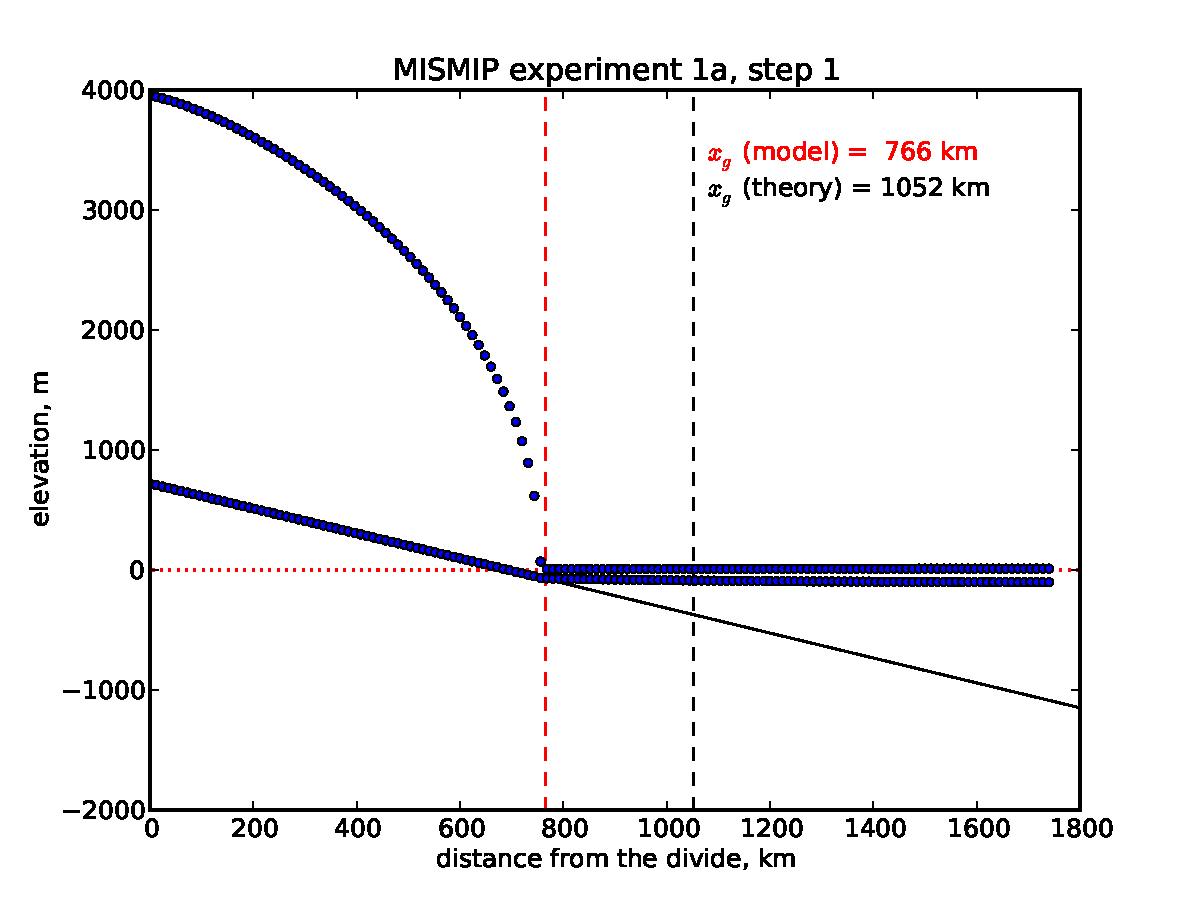
\includegraphics[width=4.0in,keepaspectratio=true]{CKH1-1a-M1-A1-profile}
\caption{A marine ice sheet profile in the MISMIP intercomparison; PISM model 1, experiment 1a, grid mode 1, step 1. Starting from a uniform $10$ m ice thickness.}
\label{fig:MISMIPmodel1exper1aM1A1}
\end{figure}

The implementation of MISMIP in PISM conforms fairly closely to the intercomparison description.  However, that document specifies
\begin{quotation}
\dots we require that the rate of change of grounding line position be $0.1$ m/a or less, while the rate of change of ice thickness at each grid point at which ice thickness is defined must be less than $10^{-4}$ m/a \dots
\end{quotation}
as a standard for ``steady state''. PISM does not include a stopping criterion such as ones described here. However, we report enough information, in PISM output files with scalar and spatially-variable time-series, to compute a grounding line rate or the time at which the thickness rate of change drops below $10^{-4}$ m/a.

One of the physical parameters regarding PISM's ice shelf model needs comment: we make the base of the ice shelves have very small resistance, using $10^{-4}$ times the linear drag typical of a Siple coast ice stream \cite{HulbeMacAyeal}, because this seems to have the effect of stabilizing the ice shelf.

\begin{figure}[ht]
\centering
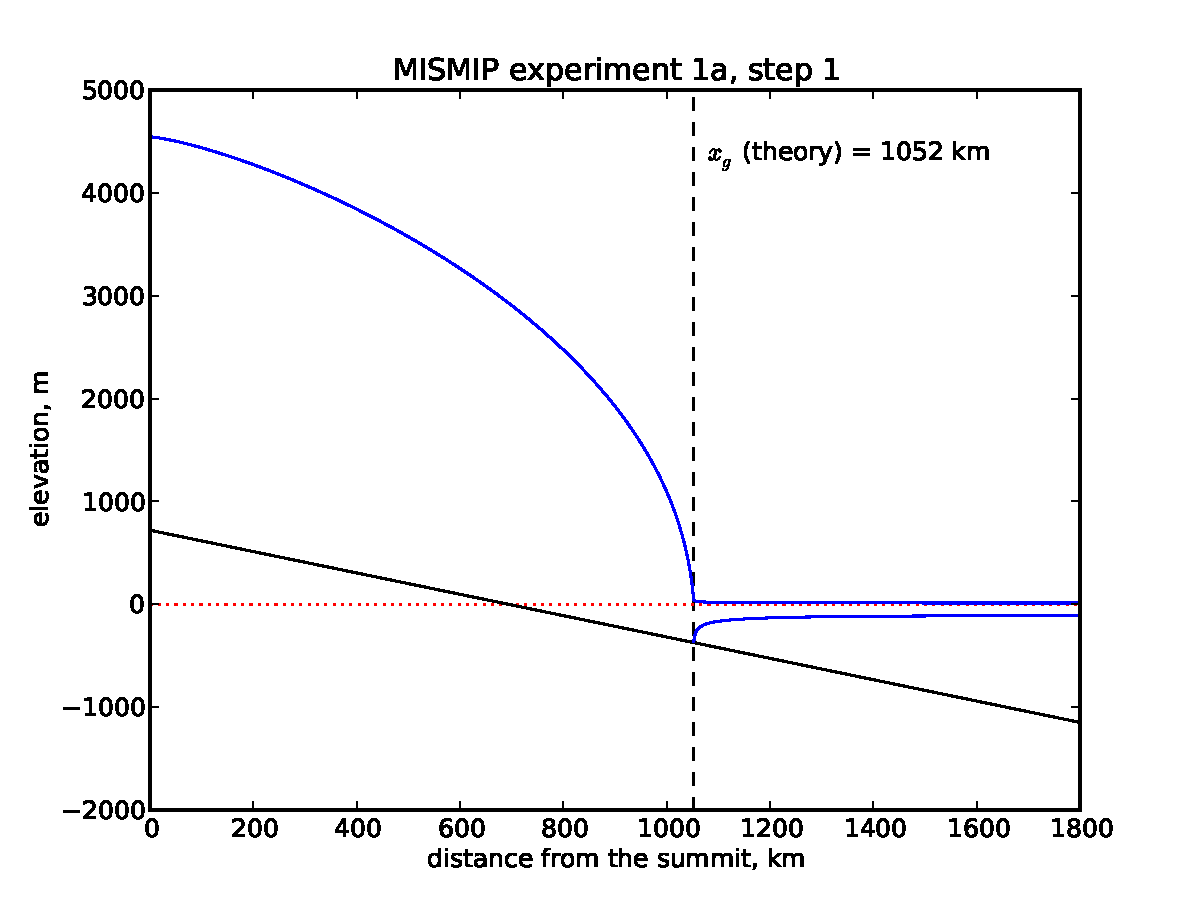
\includegraphics[width=4.0in,keepaspectratio=true]{SM-1a-A1}
\caption{Analytical profile for steady state of experiment 1a, grid mode 1, step 1, from theory in \cite{SchoofMarine1}.  This is a boundary layer asymptotic matching result, but not the exact solution to the equations solved numerically by PISM. Compare Figures \ref{fig:MISMIPmodel1exper1aM1A1} and \ref{fig:MISMIPmodel1exper1aM3A1FROMSM} generated by PISM.}
\label{fig:SMexper1aM1A1}
\end{figure}

The script \texttt{MISMIP.py} in \texttt{examples/mismip} has the ability to compute the profile from the Schoof's \cite{SchoofMarine1} asymptotic-matching boundary layer theory.  This script is a Python translation, using \texttt{scipy} and \texttt{pylab}, of the \Matlab codes in \url{http://homepages.ulb.ac.be/~fpattyn/mismip/MISMIP_distribution.tar}.  For example,

\begin{verbatim}
$ python MISMIP.py
\end{verbatim}

\noindent produces Figure \ref{fig:SMexper1aM1A1}.

We see immediately that the PISM result does not put the grounding line in the same location as Schoof's boundary layer theory.  We believe the problem is with PISM's numerical solution, not with that theory.  More evidence that the problem is numerical can be found by looking at the ice flux.  Using \texttt{ncview} to examine the diagnostic variable \texttt{cflx} (magnitude) in \texttt{ABC1_1a_M1_A1.nc} we see Figure \ref{fig:cflx1aM1A1}.  \emph{This is a problem with PISM}.  The flux should be a linear function.  Indeed, at steady state the flux $\bq$ solves $a=\Div\bq$ where $a$ is the accumulation rate.  In MISMIP, $a$ is the constant $0.3$ m/a, so at steady state $|\bq| = a x$, a line.

\begin{figure}[ht]
\centering
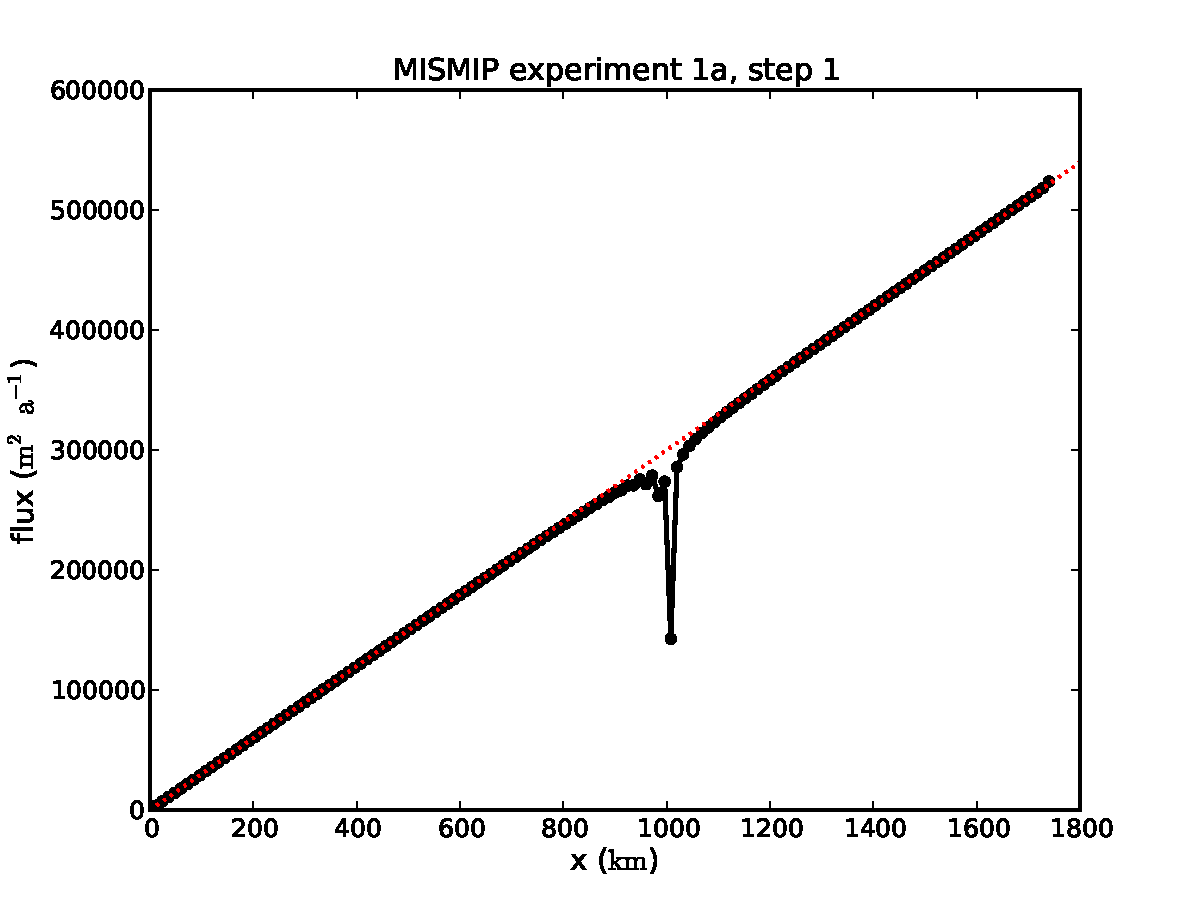
\includegraphics[width=4.0in,keepaspectratio=true]{CKH1-1a-M1-A1-flux}
\caption{Numerically computed flux $\bq = \bar\bU\, H$, where $\bar\bU$ is the vertically-averaged horizontal velocity and $H$ the thickness, for steady state of experiment 1a, grid mode 1, step 1.  Illustrates a significant numerical problem; it should be the dotted line, which has slope $a = 0.3$ m/a.}
\label{fig:cflx1aM1A1}
\end{figure}

We can learn more about the problem.  It turns out that the numerical flaw in the flux also keeps the grounding line from moving properly, we think.  The problem is that the numerical result doesn't move the grounding line to its correct location if the ice sheet and shelf are initially $10$ m as specified in MISMIP.  On the other hand, the correct location for the grounding line is also approximately a steady state for PISM numerics; the grounding line stays where you put it (compare \cite{SchoofMarine2} and \cite{VieliPayne}).

In fact, by default \texttt{run.py} uses the asymptotic-matching thickness result from the \cite{SchoofMarine1} theory to initialize the initial ice thickness, as allowed by the MISMIP specification.

The effect when we do this at higher resolution (grid mode 3 with 6km spacing, instead of 24 km), is a step forward.
The result, Figure \ref{fig:MISMIPmodel1exper1aM3A1FROMSM}, is more satisfactory.  On the other hand, inspection of the flux for this new run shows a smaller, but similarly worrying, jump in flux.

\begin{figure}[ht]
\centering
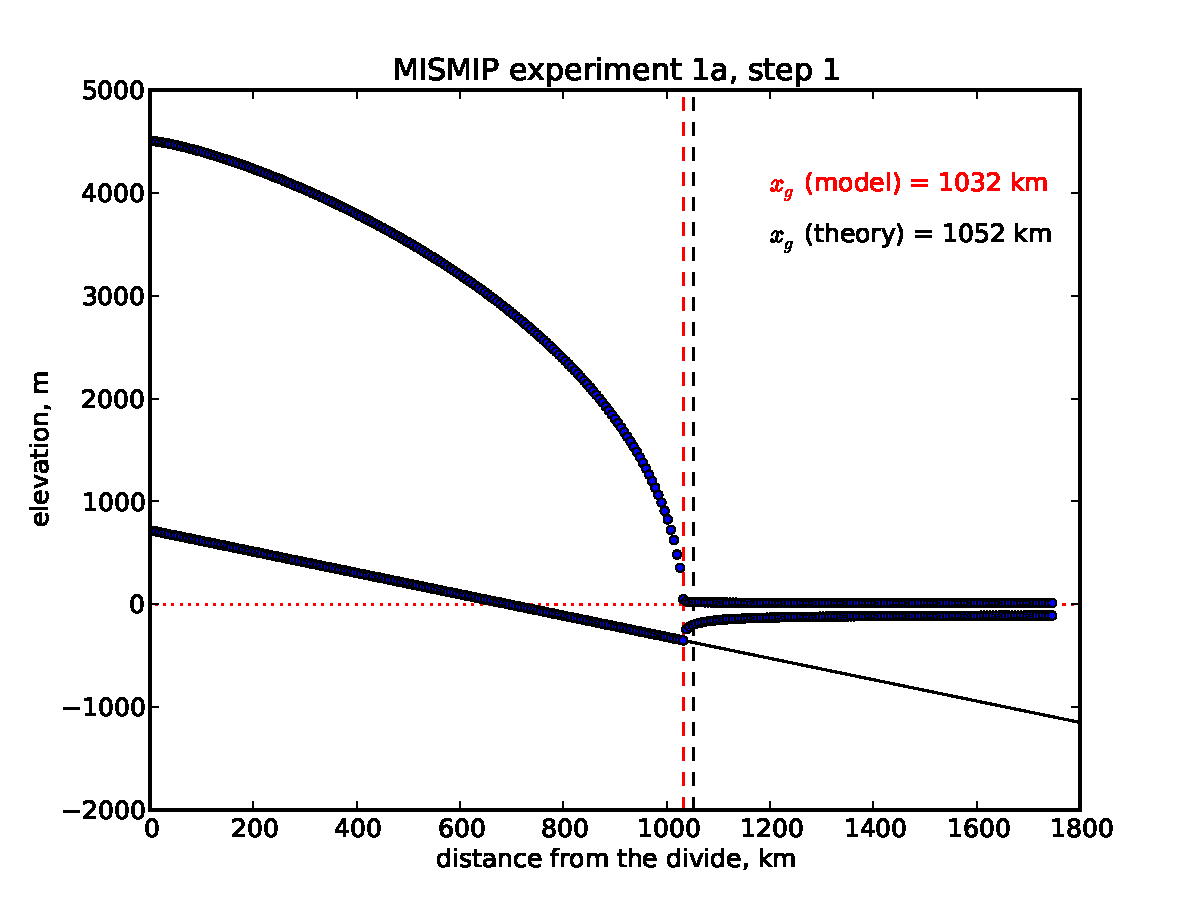
\includegraphics[width=4.0in,keepaspectratio=true]{CKH1-1a-M3-A1-profile}
\caption{A marine ice sheet profile in the MISMIP intercomparison; PISM model 1, experiment 1a, grid mode 3, step 1, but on a run started from the corresponding asymptotic-matching result.  At least the location of the grounding line agrees more closely with that in Figure \ref{fig:SMexper1aM1A1}.}
\label{fig:MISMIPmodel1exper1aM3A1FROMSM}
\end{figure}


%%% Local Variables: 
%%% mode: latex
%%% TeX-master: "manual"
%%% End: 
